\documentclass[11pt]{article}
\usepackage[a4paper, hmargin={2.8cm, 2.8cm}, vmargin={2.5cm, 2.5cm}]{geometry}
\usepackage{eso-pic} % \AddToShipoutPicture
\usepackage{graphicx} % \includegraphics
\usepackage{listings}
\usepackage{setspace}
\usepackage{cite}
\usepackage{stmaryrd}
\usepackage{fixltx2e}
\usepackage{amsmath}
\usepackage{tabu}

\lstset{
  mathescape,
  moredelim=[is][\underbar]{_}{_}
}

\definecolor{Background}{rgb}{0.98,0.98,0.98}
\lstset{
    numbers=left,
    numberstyle=\footnotesize,
    numbersep=1em,
    xleftmargin=1em,
    framextopmargin=2em,
    framexbottommargin=2em,
    showspaces=false,
    showtabs=false,
    showstringspaces=false,
    frame=l,
    tabsize=4,
    % Basic
    basicstyle=\ttfamily\small\setstretch{1},
    backgroundcolor=\color{Background}
}

\author{
  \Large{Anna Sofie Kiehn and Henriks Urms}\\
  \\ \textit{Supervisor:} Martin Elsman
  % \texttt{a.kiehn89@gmail.com} \\
  %\\ \texttt{a.kiehn89@gmail.com} \\ \\
  %\Large{Henriks Urms}
  %\\ \texttt{urmshenrik@gmail.com}
}

\title{
  \vspace{5cm}
  \Huge{Midvejsrapport} \\
  \Large{Compiling TAIL to Futhark}
}

\begin{document}
%\renewcommand{\arraystretch}{1.2}

\newcommand{\evals}[1]{\llbracket #1 \rrbracket}

%% Change `ku-farve` to `nat-farve` to use SCIENCE's old colors or
%% `natbio-farve` to use SCIENCE's new colors and logo.
\AddToShipoutPicture*{\put(0,0){\includegraphics*[viewport=0 0 700 600]{include/natbio-farve}}}
\AddToShipoutPicture*{\put(0,602){\includegraphics*[viewport=0 600 700 1600]{include/natbio-farve}}}

%% Change `ku-en` to `nat-en` to use the `Faculty of Science` header
\AddToShipoutPicture*{\put(0,0){\includegraphics*{include/nat-en}}}

\clearpage\maketitle
\thispagestyle{empty}

\newpage

\abstract

\newpage

\tableofcontents

\newpage

%%%%%%%%%%%%%%%%%%%%%%%%%%%%%%%%%%%%%%%%%%%%%
%%%%%%%%%%%%%%%%%%%%%%%%%%%%%%%%%%%%%%%%%%%%%
%%%%%%%%%%%  REPORT STARTS HERE  %%%%%%%%%%%%%%%%%%%%
%%%%%%%%%%%%%%%%%%%%%%%%%%%%%%%%%%%%%%%%%%%%%
%%%%%%%%%%%%%%%%%%%%%%%%%%%%%%%%%%%%%%%%%%%%%
\section{Prelude}

In the prelude part of this paper we try to meet the requirements of the "midtvejsrapport" assignment.
After the prelude section this rapport contains draft versions of the final report. Some of these sections are further
along than other so please keep in mind that the sections are draft and not a finished product.
Some of the sections only contain a short description of what we expect the final sections should contain, however we still have
the section in place to get an idea of the structure of the final report.  

\subsection{Problem Definition}
Is it possible, effectively to compile TAIL programs, produced by the APL compiler AplTail,
into Futhark programs and thereby make use of the Futhark infrastructure for optimization
and the possibility for targeting parallel hardware?

\subsection{Problem clarification}
The language APL is a mature array programming language that gives rise to parallelism.
The AplTail compiler produces a typed intermediate language TAIL from APL source code \cite{ElsmanDybdal:Array:2014}.
The purpose of the Futhark language is to make it possible for the programmer to express parallelism in a high level language
while at the same time targeting parallel architectures \cite{TroelsHenriksen}.
We wish to assess the possibility of compiling TAIL to Futhark thereby making it possible to execute APL in parallel
by using the Futhark language as backend.
This also allows us to take advantage of the various optimizations that Futhark provides, most notably fusion \cite{TroelsHenriksen}.

The challenges of mapping TAIL to Futhark lie mainly in the differences between how the two languages express parallelism.
The TAIL the parallelism is always flat, even for multi-dimensional arrays where as Futhark permits nested parallelism but always
does so at the level of arrays\cite{ElsmanDybdal:Array:2014} \cite{TroelsHenriksen}.

We will not test the produced code on parallel hardware as no parallel backend for Futhark yet exists.

\subsection{Methods and tools}
In this section we will describe the methods and tools used to create the compilation scheme and implementation of the compiler. 

\subsubsection{Symbolic notation to describe the compilation scheme}
We are going to use a symbolic notation to illustrate a compilation scheme showing the compilation in a way
that abstracts away implementation details \cite{MartinElsmanNotation}.
We use this tool to create a description of the compilation scheme that is independent of the implementation and
which should make it possible to implement the compiler in any language.

\subsubsection{Parser}
We used a parser that was created during an earlier project \cite{APLACC} instead of creating our own.
This was done in order to use already existing tools and save our resources for work that had not already been done by others.
We did however have to update the parser a little as it was a few months old and therefore did not support the
newest additions to the TAIL language.
Details about this implementation can be found in the section \textit{Implementation of the compiler}. 

\subsubsection{Language used}
The implementation of the compiler is written in the programming language Haskell.
We chose to write in Haskell because it is a functional language that is suitable for creating a compiler because of the 
pattern matching feature and the ease with which one can recursively go through the thee structure that 
represents the program code. Haskell has more features and libraries than Standard ML and that is why it was chosen. 

\subsubsection{Libraries used}

In our implementation we have used various external libraries, we will discuss some of the non-standard used libraries here.
For building our project and managing external libraries we have used the cabal package \cite{cabal}. This is a very common thing to
do in Haskell projects and should make it easy for anyone to build our code.
We use the tasty package \cite{tasty} which provides a test framework that we use to implement our tests. Furthermore we have used the
package tasty-golden \cite{tasty-golden} which is a plug-in for the tasty framework that allows to test against "golden" files.
A lot of projects implement their own test frameworks and we could have done the same.
We chose not to do so as this freed us to use our resources on developing the compiler instead of developing and maintaining a
test framework which could prove time consuming.
Finally the existing parser for TAIL makes use of the popular parsec library \cite{parsec} and we have continued to use
parsec in our continuation of the parser.

\subsubsection{Testing}

We provide a test suite for testing of our compiler.
Each test compiles an TAIL program and tries to run it in the Futhark interpreter and the matches the result against a reference
value found in a file with the extension ok.
This testing procedure makes sure that our compiler produces valid Futhark code from our test programs.
Most of the tests are generated from APL code with the AplTail compiler.

We also plan to provide benchmarks that test the speed of our code in the future.

\subsection{Project status}
The project is coming along as planned and we are on schedule which can be seen in Figure \ref{fig:gantt}.
It took less time than expected to adapt the parser to work with the latest version of TAIL
which meant that we started on the implementation of the TAIL functions in the compiler a few days before scheduled. 
We are done with implementing half of the functions in TAIL to Futhark source code.
As we are working on testing the implementation while we develop we are halfway through testing the functionality as well. 

\begin{figure}%[width=\textwidth]%[p]
    \centering
    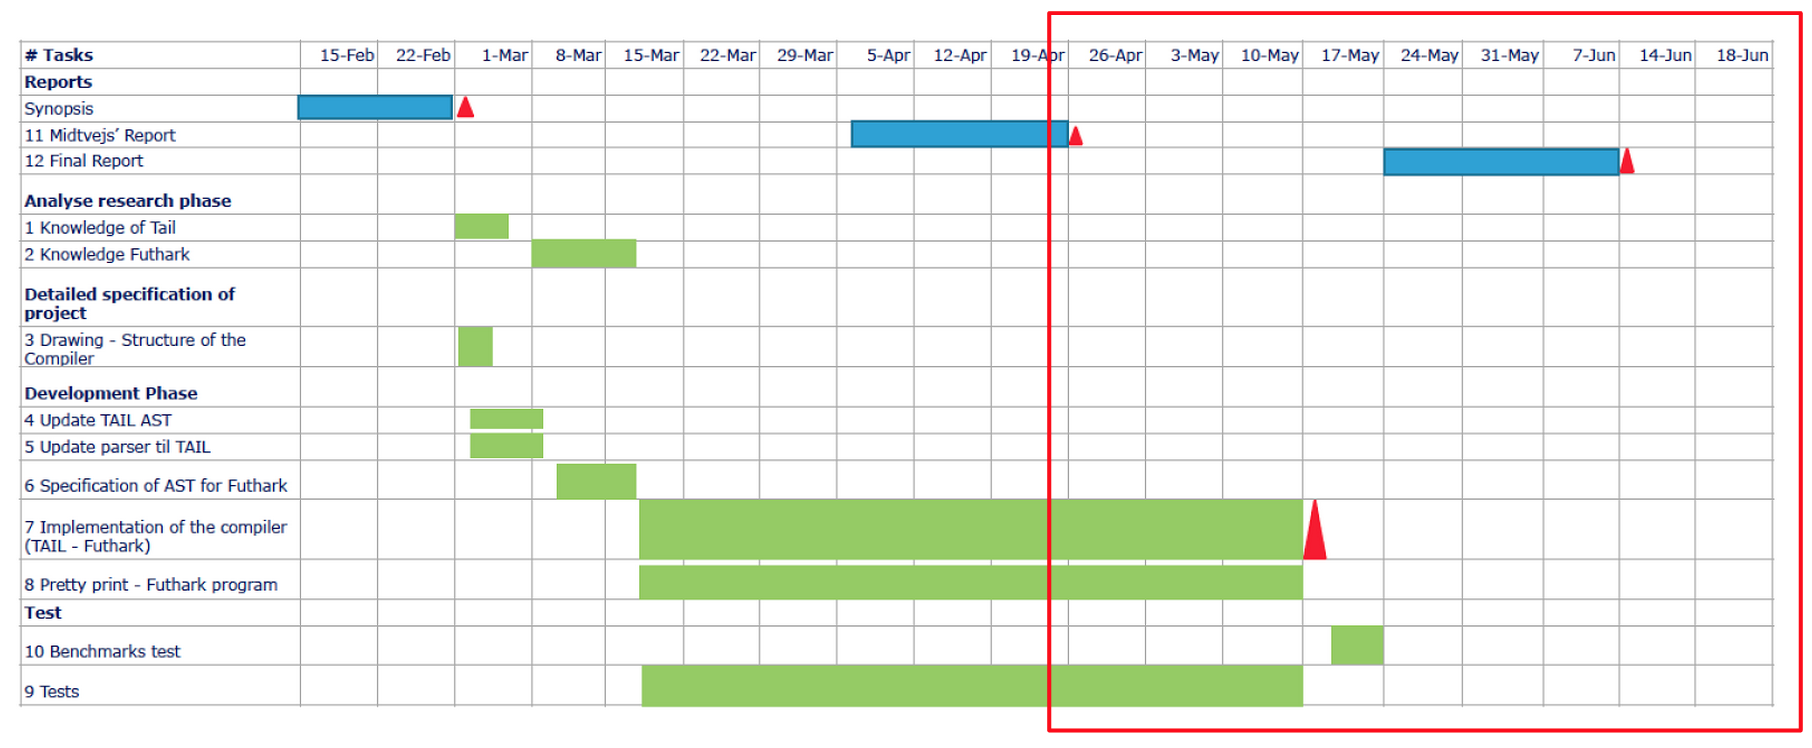
\includegraphics[width=\textwidth]{midvejsgantt3.png}
    \caption{Gantt chart of the project activities. The remaining time of the project is highlighted by a red box.}
    \label{fig:gantt}
\end{figure}

The compilation scheme we are going to create are still being developed.
The symbolic notation is something we will work intensively on from now on.
So far only a small portion of the compilation has been written in a symbolic notation,
the rest is still described in a more informal text form.
We will use the remaining time in the project focus on getting the last functions implemented and tested.

We will also test the efficiency of our generated Futhark code using benchmarks to compare it to the C-code generated by the TAIL compiler. 


\newpage

\section{Introduction}

In recent years, there has been a lot of focus on leveraging the power of parallel hardware. 
One approach has been to design programming languages with explicit data-parallel constructs that can be compiled 
into highly parallel code. One such language is Futhark. The aim of Futhark is to target parallel hardware such as 
GPUs while itself being the target of more programmer-productivity oriented languages. The Futhark compiler 
performs several optimizations, such as fusion, which enhance the degree of 
parallelism \cite{T.Henriksen&C.Oancea}.\\

APL is an array language and includes various operations that are central to the language and are good candidates 
for parallel execution. Efforts in compiling APL to parallel backends already exist in the form of the language 
TAIL (Typed array intermediate language) and it’s compiler \cite{ElsmanDybdal:Array:2014}.
The TAIL compiler captures the parallelism inherent in APL source code and brings it to a much more manageable form.
In our work we provide a compiler from TAIL 
to Futhark thus bridging the gap between APL and Futhark.\\

The language Futhark is designed to target parallel architectures and at the same time acting 
as an intermediate language for more feature-rich languages. By compiling APL to Futhark through TAIL the 
Futhark compiler can be used to generate parallel code from APL once a parallel backend for 
Futhark is completed.\\

There are traditionally five stages of a compiler if you compile a high level language to machine code: 
lexical analysis, syntax analysis, type checking, intermediate code generation, register allocation, machine 
code generation and assembly and linking \cite{TorbenMogensen}. However, in this project we are compiling from 
one high level language to another high level language. The structure does therefore look a little different. 
The first two phases are still lexical analysis and syntax analysis and are handled by a parser.
We made use of an already existing parser \cite{APLACC} and only modified it in order for it to work on the latest 
version of TAIL. The third phase is transforming the abstract syntax tree of TAIL to the abstract syntax tree 
representing the code in Futhark and the fourth phase is printing the AST so it becomes correct 
Futhark source code. \\

One of the main point of interest in the compilation between TAIL and Futhark is compiling the four array operators 
of TAIL: {\tt each}, {\tt eachV}, 
 {\tt reduce} and {\tt zipWith} to Futhark source code that include the four second-order array combinators in Futhark:  
 {\tt map}, {\tt filter}, {\tt reduce} and {\tt scan} \cite{ElsmanDybdal:Array:2014}\cite{TroelsHenriksen}. 
However as the functionality of these functions are not completely 
identical the work lies in creating a mapping that retains the parallelism in the original code in the target language.\\
This can be seen in the example below which illustrate this difference. The reduce function in the
TAIL language is mapped to a nested reduce function in the Futhark language.
As some function names exists in both languages the Futhark version of such occurrences are \underline{underlined}.

\begin{lstlisting}[numbers=none,frame=none]
reduce(+, [[1,2,3,4],[5,6,7,8]]))

  =>

_reduce_(fn x => map(+,x),[[1,2,3,4],[5,6,7,8,]])

\end{lstlisting}

This paper contributes with a compilation scheme that are implementation independent, showing a replicable 
way of how to translate the typed intermediate language of APL, TAIL, to the functional language Futhark. Also 
this paper presents an implementation of the previous mentioned scheme in Haskell. The efficiency of this
 implementation have been tested by comparing benchmarks test on code generated by the C-backend to TAIL 
 and the generated Futhark source code by using the C-backend to Futhark. \\

The project is open source and the source code can be found here:\\ https://github.com/henrikurms/tail2futhark.

\section{TAIL}

TAIL is a typed array intermediate language and the target of an APL compiler.
APL is an older language created in the 1960's by Kenneth E. Iverson.
APL is an array programming language, its main type is the multi-dimensional array 
and most of the built-in functions in the language are array operators that work on this type. 
All of its built-in functions or operators are represented by unicode symbols allowing for very concise code.
The APL language is dynamically typed. It supports first and second order functions and it supports polymorphism in 
both its first and second order functions and operators. 
Even though it is not a new language it is still used in the financial world 
where large code bases are still operational and actively developed \cite{ElsmanDybdal:Array:2014}. \\

% TAIL does not support curried functions. 

TAIL was designed with the purpose of targeting parallel architectures, though no parallel backend for TAIL yet exists.
Another backend to TAIL exists however which compile TAIL efficiently into a C-like language. TAIL does not support
 all APLs operators but only a subset of these \cite{ElsmanDybdal:Array:2014}.\\

A TAIL programs always consist of a single expression. An expression can then be a value, variable, 
list of expressions, a let expression or an operator. \\

TAILs type system takes the parallelism of APL and transforms it to a more manageable form adding explicit type
 information to the constructs.
Another benefit of the expressivity of TAILs type system is that it allows the (TAIL) compiler to express some operators which
are primitive in APL using simpler operators, one such operator is that of the inner product \cite{ElsmanDybdal:Array:2014}. \\
 
Most of the operators in TAIL are polymorphic in respect to array ranks and base types.
Some of them only take some polymorphic arguments but also take specific type arguments.
An example is the {\tt take} function. It takes as argument a number (of type int) and an array of type $\alpha$.\\

The central type in TAIL is, like in APL, the multi-dimensional array type.
Array types consist of a base type and a rank.
The base type of an array is the type of the elements in the array and can currently be of the
type: {\tt int}, {\tt double}, {\tt bool} {\tt char}. 
Scalars are a special case of the array type and is represented as an array of rank 0. 
Vectors can be represented in two different ways in TAIL.
Either as an array of rank 1 or as the special vector type.
The special vector type is used for vector literals where the length of the vector is known at compile time \cite{ElsmanDybdal:Array:2014}. \\


There are four parallel operators in TAIL, {\tt each}, {\tt eachV}, {\tt reduce} and {\tt zipWith}.
The functions {\tt each} and {\tt eachV} are known in many languages as map.
The function takes two arguments: a function and an array and then apply this function on the array.
If the rank of the array is greater than 1 the {\tt each} function work as a map on the fattened representation of the array,
that is, the function is applied on the inner most dimension of the array.
The {\tt eachV} function is a special case of {\tt each} and is used on the special vector type.\\

The function {\tt reduce} works similar to fold known in functional languages.
Their function takes as arguments a associative binary operator, a neutral element and array.
The {\tt reduce} function the uses the binary operator 
to reduce an array of rank $\gamma+1$ to an array of rank $\gamma$ by reducing along the inner-most dimension.
The difference to fold is that the operator has to be associative and the start element has to be neutral
because the execution is parallel.

The {\tt zipWith} function takes as arguments a function and two arrays.
It then applies the function on the pair of elements consisting of the i'th element
from the first array and the i'th element from the second array.
Like the other tree operators it works on the inner-most dimension of the array\cite{ElsmanDybdal:Array:2014}\cite{TorbenMogensen}. \\

%%If we do not show the type schemes here we should reference to where they can be found in the article!!!!!!!!!!

%The types in TAIL are divided into four types. Firstly there are base types consisting of {\tt int}, {\tt double}, {\tt bool} and the polymorphic type {\tt $\alpha$} that can represent any one of them. Secondly, there are shape types that can be either a scalar value/variable of type int,  or a shape variable or a combination of two shape variables. \\
%Then there is array types that consist of a base type and a rank. Finally there is 


%The main datatype in TAIL is also a multidimensional array. Array types are in TAIL annotated with their ranks explicitly. 
%TAILs type system treats scalar values as special cases of the array time namely an array with rank 0. 

%There are two separate representations of vectors, either the special vector type used when the length of the vector is known or the general array type where the rank is 1.  
 
%Besides array and vector types, TAIL also have base types in the form of {\tt int}, {\tt double}, {\tt bool} and {\tt $\alpha$}.

%So far TAIL only support a subset of the APL functions and operators. 

\section{Futhark}

Futhark is a functional programming language inspired by Haskell and Standard ML.
It was designed to be an attractive choice for expressing complex programs by having enough expressive power without
losing the possibility to do aggressive optimization and creating parallelism even though the higher the expressive power of the
language the more difficult optimization often become.
Due to the focus on optimization the Futhark language only supports regular arrays
(arrays where all inner dimensions are of the same length)
because of the complication to size analysis supporting non-regular arrays would create.
However Futhark do support nested parallelism as this is a feature many programs 
depend upon even though this feature does make optimization more difficult \cite{TroelsHenriksen}.

%%something more about specific optimization????????????????\\


A Futhark program consist of a list of function declarations of the form:
\begin{lstlisting}[numbers=none,frame=none]
fun return-type name(params...) = body
\end{lstlisting}

The body of the Futhark function then consist of an expression.\\

The Futhark language support anonymous functions, but it is not possible to curry functions in the Futhark language,
so the anonymous function can only take one argument.
If the function needs more than one argument it needs to be given as a tuple.
Except for inline anonymous functions all functions are defined globally \cite{TroelsHenriksen}. \\

The Futhark language supports multidimensional arrays in the form of nesting of array types,
i.e. an int array array will contain int arrays and so on.
The Futhark language has four base types: {\tt int}, {\tt real}, {\tt char} and {\tt bool}.
In general the Futhark language does not support polymorphism in functions,
the only exception is the built-in second-order array combinators that work on arrays of any base type. \\

Futhark is mostly a first order language but supports bulk (parallel) operations on arrays
using the built-in second-order array combinators (SOACs) of the language. 
The SOACs consist of {\tt map}, {\tt filter}, {\tt reduce} and {\tt scan}.
The operators have the expected functionality also found in Haskell and Standard ML,
that is {\tt map} takes a function and an array and apply the function on the array.
If the array is multi-dimensional the function is applied to the outer most dimension.
The function {\tt reduce} takes as arguments a function, a neutral element and an array.
Like the {\tt map} function, the {\tt reduce} function takes the function it is given in the arguments
and apply it on the outer-most dimension of the array \cite{TroelsHenriksen}. \\ 

%The basic types in Futhark is {\tt int}, {\tt char}, {\tt bool}, {\tt real} and regular arrays.
%The type system of Futhark does not support polymorphism,
%however the build-in SOACs work on all regular arrays created of the basic types. 

%Does not support polymorfism in types

\section{The differences between TAIL and Futhark}
In this section we are going to flesh out the concrete differences between the two languages. 

The differences in how Futhark and TAIL handles parallelism is tightly connected with the differences in their type systems.
Multi-dimensional arrays in TAIL are typed by a base type and a rank. The array operators of TAIL are polymorphic in the rank
of the array. This means that the operators that the array operators take as arguments always work on base types \cite{ElsmanDybdal:Array:2014}. In contrast
arrays in Futhark can be of any type, even other arrays. Arrays of arrays are how multi-dimensional arrays are represented in Futhark.
This means that the SOACs in Futhark can apply the functions they take as arguments to arrays themselves, these functions can then
map other functions and so on, this leads to nested parallelism \cite{TroelsHenriksen}.
%\subsection{Polymorphism}

\section{Compilation strategy}
In this section we are going to introduce our compilation scheme and explain the problems in compiling the different functions
having a special focus on the more interesting cases.
We will also explain our reasoning behind the chosen compilation and what alternatives there are.

Below we introduce a scheme of the compilation from TAIL to Futhark. The scheme uses a mathematical notation to illustrate
the compilation of the TAIL expressions to Futhark code/expressions?


This scheme works as an abstract model of the transformation and is implementation independent. It is based on similar schemes \cite{MartinElsmanNotation} . \\

The TAIL language consist of the following expressions \cite{ElsmanDybdal:Array:2014}: 

\begin{lstlisting}[numbers=none,frame=none]
e$_T$ ::= x | i | d | c | inf | -e | let x:t = e$_1$ in e$_2$ |
      op[e$_1$,...,e$_n$] | fn x:t e | [e$_1$,...,e$_n$]
      
\end{lstlisting}

The Futhark language consist of the following expressions\cite{TroelsHenriksen}: 
\begin{lstlisting}[numbers=none,frame=none]
e$_F$ ::= 
      
\end{lstlisting}

The compilation between these two languages can be seen below: \\


%%% Table
\begin{tabular}{l c l}% to \linewidth {l c X}
$\evals{x}$ & $=$ & $x$ \\
$\evals{i}$ & $=$ & $i$ \\
$\evals{d}$ & $=$ & $d$ \\
$\evals{c}$ & $=$ & $c$ \\
$\evals{-e}$ & $=$ & -$\evals{e}$ \\
$\evals{ \text{let } x:t = e_1 \text{ in } e_2} $ & $=$ & let $\evals{x} = \evals{e_1} \text{ in } \evals{e_2} $\\
$\evals{[e_1,...,e_n]}$ & $=$ & $ [ \evals{e_1},...,\evals{e_n}]$\\
$\evals{\text{op } [e_1,...,e_n]}$ & $=$ & $\evals{\text{op}}_{op} \evals{[e_1,...,e_n]}$\\

$\evals{\text{op} [e_1,...,e_n]}$ & $=$ & $\evals{\text{op}}_{fun} \; (\evals{e_1},...,\evals{e_n})$\\
$\evals{\text{op} [e_1,e_2]}$ & $=$ & $\evals{e_1} \; \evals{\text{op}}_{op} \; \evals{e_2}$\\

$\evals{\text{each}_{[t_1,t_2,r]}(f,a)}$ & $=$ & $
  \begin{cases}
    $map$(\evals{f}_{fn}^{\evals{t_2}},\evals{a}) & r=1\\
    $map (fn $t_2^r \; (t_1^r \; x)$ {\tt =>} $ \evals{\text{each}_{[t,r-1]}(f,x)},\evals{a}) & r > 1  \\
  \end{cases}$\\

$\evals{\text{eachV}_{[t_1,t_2,r]}(f,a)}$ & $=$ & map$(\evals{f}_{fn}^{\evals{t_2}},\evals{a}) $  \\         

$\evals{\text{vrotate}_{[t,r]}(i,a)}$ & $=$ & map(fn x {\tt =>} a[x + i {\tt \%} \text{size}(0,a)], iota(size(0,a)) \space\space , x = fresh\\
$\evals{\text{vreverse}_{[t,r]}(a)}$ & $=$ & map(fn x {\tt =>} a[\text{size}(0,a)-x-1], $\text{iota}(\text{size}(0,a))$ \space\space , x = fresh\\
$\evals{\text{reshape}_{[t,r_1,r]}(a_1,a_2)}$ & $=$ & reshape$(\evals{a_1},(\text{reshape1}_{\evals{t}}(
% \prod_{i=0}^{r_1} \text{size}(i,a_1)
\text{osize}%(\text{size}(0,a_1)*\ldots*\text{size}(r_1,a_1)
, \text{reshape}(
\text{isize}%\text{size}(0,a_2)*\ldots*\text{size}(r_2,a_2)
, \evals{a_2})))) $ \\
&& \hspace{4ex} where osize = $\text{size}(0,a_1)*\ldots*\text{size}(r_1,a_1)$ \\
&& \hspace{4ex} \phantom{where} isize = $ \text{size}(0,a_2)*\ldots*\text{size}(r_2,a_2) $ \\

$\evals{\text{reduce}_{[t,r]}(f,n,a)}$ & $=$ & $
  \begin{cases}
    \text{reduce}(\evals{f}_{fn}^{\evals{t}},\evals{n},\evals{a}) & r=1 \\
    $map (fn $ t^{r-1} \; (t^r \; x)$ {\tt =>} $ \evals{\text{reduce}_{[t,r-1]}(f,n,x)},\evals{a}) & r>1\\
  \end{cases}$\\

$\evals{\text{zipWith}_{[t_1,t_2,t_3,r]}(f,a_1,a_2)}$ & $=$ & \\
  \multicolumn{3}{r}{ $\begin{cases}
    $map$(\evals{f}_{fn}^{\evals{t_3}},$zip($\evals{a_1},\evals{a_2})) & r=1 \\
    $map(fn $t_3^{r-1} \; (t_1^{r-1} \; x, t_2^{r-1} \; y) $ {\tt =>} $
      \evals{\text{zipWith}_{[t_1,t_2,t_3r-1]}(f,x,y)} , $zip($ \evals{a_1}, \evals{a_2})) & r>1\\
  \end{cases}$ }\\

$\evals{\text{cat}_{[t,r]}(a_1,a_2)}$ & $=$ & $
  \begin{cases}
    \text{concat}(\evals{a_1},\evals{a_2}) & r=1 \\
    $map (fn $ \evals{t}^{r-1} \; (\evals{t} \; x, \evals{t} \; y)$ {\tt =>} $ \evals{\text{cat}_{[t,r-1]}(x,y)}, \text{zip}(\evals{a_1}, \evals{a_2}) & r>1\\
  \end{cases}$\\

$\evals{\text{first}_{[t,r]}(a)}$ & $=$ & let x = $\evals{a}$ in $x[\underbrace{0,...,0}_\text{r times}]$\\

$\evals{\text{firstV}_{[t,r]}(a)}$ & $=$ & $\evals{\text{first}_{t,1}(a)}$\\

$\evals{\text{take}(i,a)}$ & $=$ & reshape(oshape,\text{take1}$_{\evals{t}}$(osize,\text{reshape}(isize,$\evals{a})))$\\
&& \hspace{4ex} where oshape = ($|i|, \text{size}(1,\evals{a}),\cdots,$size(r,$\evals{a}$))\\
&& \hspace{4ex} \phantom{where} osize = ($i* \text{size}(1,\evals{a}) *\ldots*$size(r,$\evals{a}$))\\
&& \hspace{4ex} \phantom{where} isize = \text{size}(0,$\evals{a}$)$*\ldots*$\text{size}(r,$\evals{a}$)\\

$\evals{\text{takeV}_t(d,a)}$ & $=$ & $\text{take1}_{\evals{t}}(\evals{d},\evals{a})$\\

$\evals{\text{drop}(i,a)}$ & $=$ & \text{reshape}(\text{oshape}, $\text{drop1}_{\evals{t}}(\text{osize}, \text{reshape}(\text{isize},\evals{a}))$\\
&& \hspace{4ex} where oshape = (max(0,size(0,$\evals{a}$)-$|i|$),size(1,$\evals{a}$)$,\ldots,$size(r,$\evals{a}$))\\
&& \hspace{4ex} \phantom{where} osize = ($i *$size(1,$\evals{a}$)$ * \ldots*$size(r, $\evals{a}$))\\
&& \hspace{4ex} \phantom{where} isize = \text{size}(0,$\evals{a}$)$*\ldots*$\text{size}(r,$\evals{a}$)\\

$\evals{\text{dropV}_t(d,a)}$ & $=$ & $\text{drop1}_{\evals{t}}(\evals{d},\evals{a})$\\

$\evals{\text{transp}_{t,r}(a)}$ & $=$ & rearrange$((r-1,...,0),\evals{a})$\\

$\evals{\text{transp2}_{t,r}(a_1,a_2)}$ & $=$ & let $x$ = $\evals{a_1}$ in rearrange(($x[0]$-$1,\ldots,x[r$-$1]$-$1$),$\evals{a_2})$\\

%$\evals{\text{cons}_[t,r](e,a)}$ & $=$ &  
%  $\begin{cases}
%    \text{concat}([\evals{e}],\evals{a}) & r= 1\\
%    \text{map (fn }$$(x,y) $ {\tt =>} $ \evals{\text{cons}_{[t,r]}(x,y)}, \text{ zip}(\evals{e},\evals{a}))$$ & r > 1
%  \end{cases}$\\

$\evals{\text{cons}_[t,r](e,a)}$ & $=$ & rearrange$((r,\ldots,0), \text{concat(exp,arr)})$\\
&& \hspace{4ex} where exp = rearrange((r-1,\ldots,0),$\evals{e}$)\\
&& \hspace{4ex} \phantom{where} arr = rearrange((r-1,\ldots,0),$\evals{a}$)\\
  
$\evals{\text{snoc}_[t,r](a,e)}$ & $=$ & rearrange$((r,\ldots,0), \text{concat(arr,exp)})$\\
&& \hspace{4ex} where exp = rearrange((r-1,\ldots,0),$\evals{e}$)\\
&& \hspace{4ex} \phantom{where} arr = rearrange((r-1,\ldots,0),$\evals{a}$)\\
  
%$\evals{\text{snoc}_[t,r](a,e)}$ & $=$ & 
%  $\begin{cases}
%    \text{concat}([\evals{a}],\evals{e}) & r= 1\\
%    \text{map (fn }$$(x,y) $ {\tt =>} $ \evals{\text{snoc}_{[t,r]}(x,y)}, \text{ zip}(\evals{a},\evals{e}))$$ & r > 1
%  \end{cases}$\\

$\evals{\text{iota}(a)}$ & $=$ & map$(+ \; (1), \text{iota}(\evals{a})$\\

$\evals{\text{iotaV}(a)}$ & $=$ & $\evals{\text{iota}(a)}$\\

$\evals{\text{shape}_{t,r}(a)}$ & $=$ & $[\text{size}(0,\evals{a}),...,\text{size}(r-1,\evals{a})]$\\

$\evals{\text{shapeV}_{t,r}(a)}$ & $=$ & $[r]$\\
gi
\\
%\end{tabular}\\
%
%The compilation of fn are descirbed in a table of its own\\
%
%\begin{tabular}{l c l}
$\evals{ \text{fn } x:t $ {\tt =>} $ e}^{\tau}_{fn} $ & $=$ & $ \text{fn } \tau (\evals{t}\; x) $ {\tt =>} $ \evals{e}$\\
$\evals{ \text{fn } x:t_1$ {\tt =>} $\text{fn } y:t_2 $ {\tt =>} $ e}^{\tau}_{fn} $ & $=$ & $ \text{fn } \tau (\evals{t_1}\; x, \evals{t_2} \; y) $ {\tt =>} $ \evals{e}$\\
\end{tabular}\\

The gereral compilation of operators:\\

\begin{tabular}{l c l}
$\evals{addi}_{op}$ & $=$ & $+$\\
$\evals{i2d}_{fun}$ & $=$ & toReal\\ 
\end{tabular}\\

\paragraph{reshape}
reshape gets as argument the return type.\\
It is not possible to reshape something that has length 0. It is possible in aplt but we do not support it in our implementation. \\

\paragraph{cons} takes an array of rank $\gamma$ and an array of rank $\gamma+1$ and concatinates the elements of the 
array of rank $\gamma$ in the front of the elements of the array of rank $\gamma +1$. This result in an array of rank $\gamma+1$. 
The idea behind the compilation of the function snoc was to transpose the two arrays, then concating the arrays and then transposing the resulting array again. That way we would get the desired result of the nth elements from the first array added to the nth element of the second array. However the Futhark transpose function differs slightly from the wished functionality in that. ...\\

As mentioned previously a Tail program always consists of a single expression,
whereas a Futhark program is a list of function declarations.
The Tail expression is therefore translated/compiled to a Futhark expression by making it the body of the Futhark function\cite{ElsmanDybdal:Array:2014}\cite{TroelsHenriksen}. 
Thus the focus should be on translating Tail expressions to Futhark expressions. 
There are 10 different kind of Tail expressions most of which has exact equivalents in the Futhark language.
This includes but are not limited to, variables, let expressions and literals.
Thus the interesting case is really when the expression to compile is an operator expression. \\

These operators consist of the scalar operators: add, addi, subi, subd, multi, multd, mini, mind, maxi, maxd, andb, orb, xorb, nandb, norb, notb, lti, ltd, ltei, lted, gti, gtd, gtei, gted, eqi, eqd, negi, negd, i2d and b2i, and the array operators: iotaV, iota, eachV, each, reduce(V), reduce, shapeV, shape, reshape, reshape0, reverse, vreverse, rotateV, vrotateV, rotate, transp, transp2, takeV, take, dropV, drop, consV, cons, snocV, snoc, firstV, first, zipWith, catV and cat \cite{ElsmanDybdal:Array:2014}. \\

Most of the scalar operators have equivalents in the Futhark language and are therefore straight forward to compile.
Some of the Tail array operators also have equivalent or almost equivalent counterparts in the Futhark language
but most have not and are therefore interesting to take a closer look at.


\section{The parallel operators}

\subsection{each}

The type scheme of the {\tt each} function is $each(f,a) :: \forall\alpha\beta\gamma.(\alpha \to \beta) \to [\alpha]^\gamma \to [\beta]^\gamma$.

The {\tt each} function in TAIL applies a function to every element in the flat representation of the array.
This is a completely parallel operation more commonly known as map.
The {\tt map} combinator in Futhark has slightly different semantics\cite{ElsmanDybdal:Array:2014}.
Since Futhark views a multidimensional array as nested simple arrays it applies the function to every array element.
That is, it maps the function into the outer-most dimension of the array\cite{TroelsHenriksen}.

To solve this problem we have nested {\tt map}s to the depth of the array with the required function,
for example, an {\tt each} operation over an array of rank 2 would have two {\tt map}s nested in each other so the kernel is
mapped on each element of basic type.

For example an each operation on an array of rank 2 will look like:
\begin{lstlisting}[numbers=none,frame=none]
each(f,a)	=>	map(fn x => map (f,x), a)
\end{lstlisting}

This means the parallel {\tt each} operations in TAIL are compiled to parallel code in the Futhark language.

\subsection{eachV}
The {\tt eachV } is just a special case of the {\tt each} operator that works on vectors, i.e. flat arrays where the size
is known at compile time. We do not use this extra information so this special case is not important for us.

\subsection{reduce}
The type of the {\tt reduce} function is $reduce(f,id,a) :: \forall\alpha\gamma.(\alpha \to \alpha \to \alpha) \to \alpha \to [\alpha]^{\gamma+1} \to [\alpha]^\gamma$.
The {\tt reduce} function in TAIL uses an associative binary operator to reduce an array of rank
$\gamma+1$ to an array of rank $\gamma$ by reducing along the inner-most dimension\cite{ElsmanDybdal:Array:2014}.
The Futhark reduce on the other hand reduces each array in the outer array, i.e. it reduces along the outer-most dimension\cite{TroelsHenriksen}. 

We have adopted the same approach as with each by using nested maps to map the reduce on the innermost dimension.

Fore example reducing an array of rank 2 emits the following code:

\begin{lstlisting}[numbers=none,frame=none]
reduce(+,a)	=> 	map(fn x => _reduce_(+,x), a)
\end{lstlisting}

\subsection{zipWith}

The zipWith operator applies a scalar binary operator on pairs of elements from two arrays of the same shape two
produce a third array of the same shape as the input arrays \cite{ElsmanDybdal:Array:2014}.

To do this in Futhark we use the zip function to convert two arrays to an array of tuples and map the binary operator on that array of tuples \cite{TroelsHenriksen}.

\section{Other interesting operators}

Besides the parallel operators there are other operators worth mentioning mostly because of non trivial semantics.  

\subsection{reshape}

The reshape operator also has quite unique semantics in TAIL, if the dimensions of reshape don't match the dimensions of the array, the
array is either truncated or the elements are repeated until the array is long enough \cite{ElsmanDybdal:Array:2014}.

Futhark has a reshape function that only works for arrays of the correct dimensions \cite{TroelsHenriksen}.

Our general strategy for compiling reshape is to first ensure that the array is the correct size and then use the Futhark reshape
function to do the final step. To adjust the size we operate on the flat representation of the array, this is easy to produce also
using Futhark reshape. To adjust the array we first make sure it is long enough by extending it using the function replicate and then
truncate it to the correct length with split.

To keep the implementation simple we generate code that calls generated library functions written in Futhark which do most of the work.
Nevertheless we inline the flattening and reshaping code so we only need reshape functions written in Futhark
for the one dimensional cases. If we wanted to simply call a function instead we would need a separate library function for each
rank and basic type combination which we needed to call reshape on since Futhark only allows declaration of monomorphic functions \cite{TroelsHenriksen}.

We have to decide where to put the library functions.
We would like the compiler to always output a valid (runnable) Futhark program given a valid TAIL input program, so we would like to
be able to include the library in the output when we run the compiler.
Furthermore since Futhark has no polymorphism we have to include versions of all types, but we would like to only maintain one version.
Finally since Funthark is eventually expected to feature polymorphism and a module system we would like the solution to not be too
extensive\cite{TroelsHenriksen}. Therefore we have coded the functions in the compiler itself.

We have used this approach throughout our compiler, e.g. the take operator is implemented similarly.

\subsection{take} 

The {\tt take} operator in TAIL has very unique semantics, for a positive argument that is less than the size of the array it behaves as one would suspect i.e. it returns the first n elements of the array.
For a negative argument {\tt take} returns the last n elements of the array.
If there are not enough elements in the array, {\tt take} pads with zeros.

In a similar fashion to the TAIL {\tt reshape} function we have used library functions do most of the work.
We flatten the array, let the library function work on the flat representation and finally reshape it to the desired shape.
This approach has all the benefits mentioned earlier.

\section{Implementation of the compiler}


In this section we will present the Haskell implementation of the compiler and describe how it works.
%We will show code snippets that illustrate interesting parts of the compilation.

The compiler is made up of three parts, the parser, the compiler and the pretty-printer. Once the input is parsed into an AST the
TAIL expression represented by the AST is passed to the the compileProgram function in the file \\
{\tt src/Tail2Futhark/Compile.hs}.
This function mainly pattern-matches on the tree and in the case of an operator passes the expression to the compileOpExpression
function.
This function matches on the operator name and most operators have their own separate functions that compile them.
In the process every variable has the prefix "t\_" prepended to make sure that when we make new names they cannot clash
with the old ones as long as they don't start with "t\_".

%we expect that the terms we get in are well typed and correct. 
\subsection{Adaption of the parser}

The parser that we make use of was created in a precious project \cite{APLACC}.
In the time between that project finished and ours commenced the TAIL language
had been updated with new features and we therefore had to update the parser so that it worked with the latest version of TAIL.\\

One of the things that had changed was that booleans was added to the TAIL language. %That meant that it had to be added ..\\

Another thing that had changed was that the shape type in the older version of TAIL was replaced with a vector type in the newer version \cite{ElsmanDybdal:Array:2014}.\\

\section{Testing}
In this section we will present our testing scheme, why we have chosen to test in that way and the results of the test.\\

We have used two methods to test the compiler we have created.
One is unit or integration test where we test the entire pipeline from giving it APL source code to running Futhark source code.
The code is parsed through the APL to TAIL compiler \cite{ElsmanDybdal:Array:2014}
through our compiler (TAIL to Futhark) and then through the Futhark compiler \cite{TroelsHenriksen}.
The result is then compared to the content of a file containing the expected result.
If they match the test is positive. This form of testing will test the correctness of our code. \\

The second way is benchmark test to test efficiency. 

%The second way are going to do testing is by benchmark test. This we will do in order to evaluate the efficiency of our code. 

\section{Discussion}
In this section we will discuss benefits and drawbacks with our chosen compilation strategy.
We will discuss how thing can be improved for instance how polymorphism in Futhark could make the compilation easier.
We will also discuss the test results.
Ideas to some themes are: No polymorphism in Futhark yet makes the compilation more difficult and create a lot of duplicate code.
There are no way of really testing the generated code as no parallel backend exists for either TAIL or Futhark.

\section{Summary and future work}



%%%%%%%%%%% REFERENCES  %%%%%%%%%%%%%%

\bibliography{references}{}
\bibliographystyle{plain}

There will be more references in the final thesis. 
\end{document}
